% "{'classe':('PSI'),'chapitre':'num_ia','type':('td'),'titre':'Poulie-courroie', 'source':'CCINP PSI 2024','comp':('A3-08','C3-03'),'corrige':False}"
%\setchapterimage{fig_00.jpg}
\chapter*{TD \arabic{cptTD} \\ 
Contrôle du correcteur de facteur de puissance par Intelligence Artificielle \ifnormal $\star$ \else \fi \ifdifficile $\star\star$ \else \fi \iftdifficile $\star\star\star$ \else \fi -- \ifprof Corrigé \else Sujet \fi}
\addcontentsline{toc}{section}{Application \arabic{cptApplication} : Contrôle du correcteur de facteur de puissance par Intelligence Artificielle \ifnormal $\star$ \else \fi \ifdifficile $\star\star$ \else \fi \iftdifficile $\star\star\star$ \else \fi -- \ifprof Corrigé \else Sujet \fi}

\iflivret \stepcounter{cptTD} \else
\ifprof  \stepcounter{cptTD} \else \fi
\fi

\setcounter{question}{0}
\marginnote{CCINP -- PSI -- 2024 -- Modélisation.}
\marginnote[1cm]{
\UPSTIcompetence[2]{A3-08}
\UPSTIcompetence[2]{C3-03}
}

Le correcteur de facteur de puissance est utilisé pour minimiser les pertes en lignes engendrées par l'installation électrique d'un petit studio. 

\begin{figure}[!h]
\centering
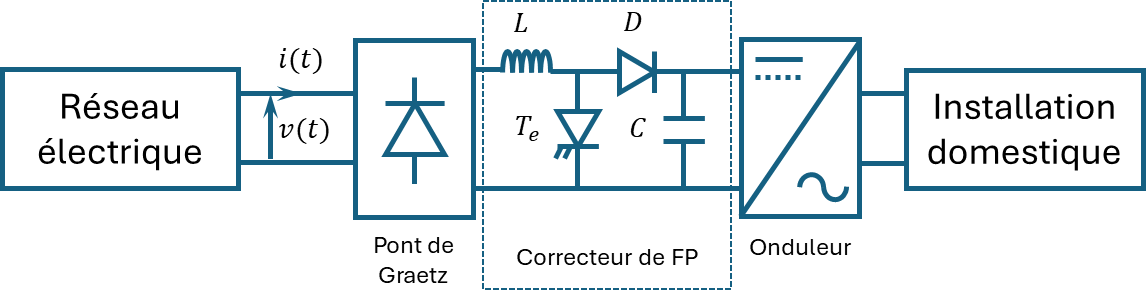
\includegraphics[width=.9\linewidth]{fig_14}
\caption{ Correcteur de facteur de puissance utilisé pour une installation domestique\label{Cy_07_ch_02_td_01_fig_14}}
\end{figure}
La figure \ref{Cy_07_ch_02_td_01_fig_14} présente le schéma de principe du dispositif complet : la tension aux bornes du condensateur $C$ est placée en entrée de l'association d'un onduleur de tension et de l'installation électrique du studio. Une boucle de régulation permet de réguler cette tensioà une valeur constante. 

L'installation étudiée comporte un ensemble box internet-télévision, un système d'éclairage, un radiateur électrique, un chauffe-eau.

*******

\subsection*{Contrôle du paramètre $\Delta$ avec un réseau de neurones}
Il faut mettre en place un contrôleur capable de fournir la consigne $\indice{\Delta}{opt}$\sidenote{A VERIFIER} en fonction des différentes combinaisons $\left(x_1, x_2, x_3, x_4 \right)$. Le contrôleur associé au correcteur de facteur de puissance doit permettre en temps réel de : 
\begin{itemize}
\item soit de désactiver le correcteur de facteur de puissance en connectant l'installation électrique du studio au réseau électrique (cas $\Delta = -1$ \sidenote{a vérifier});
\item soit de fixer de la valeur du paramètre $\Delta$ lorsque le correcteur de facteur de puissance est activé.
\end{itemize}

\begin{marginfigure}
\centering
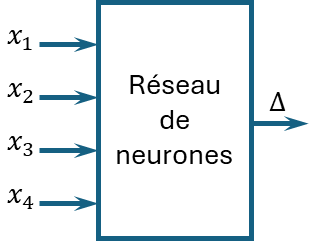
\includegraphics[width=.8\linewidth]{fig_15}
\caption{Entrées-sortie du réseau de neurones\label{Cy_07_ch_02_td_01_fig_15}}
\end{marginfigure}

Le tableau \ref{Cy_07_ch_02_td_01_tab_03}\sidenote{à récup} nous donne la correspondance entre les états des appareils $x_i$\sidenote{ verif} et le réglage $\Delta$ du correcteur. Les données d'entrainement sont celles qui vont servir à l'entrainmenet du réseau de neurons. Les données de test sont celles qui vont permettre de valider si l'entrainement s'est bien effectué. D'un point de vue système, cela revient à chercher la relation entre les données d'entrées $x_i$ et la sortie $\Delta$ (figure \ref{Cy_07_ch_02_td_01_fig_15}). 


L'objectif est de trouver un modèle de comportement qui permet, à partir du tableau \ref{Cy_07_ch_02_td_01_tab_03} de retrouver les valeurs d'entrainement et de prédire les valeurs de tests. 

Pour y ariver, l'idée est d'entrainer un réseau de neurones de manière supervisée à partir des données du tableau \ref{Cy_07_ch_02_td_01_tab_03}.

% Q31
\question{Quels sont les avantages et les inconvénients du choix d'un réseau de neurones pour modéliser la commande ?}
\ifprof
\begin{corrige}
\end{corrige}
\else
\fi

% Q32
\question{L'apprentissage supervisé est-il pertinent ? Justifier votre réponse.}
\ifprof
\begin{corrige}
\end{corrige}
\else
\fi


\subsection*{Définition d'un perceptron}

Le réseau de neurones choisi est un perceptron multicouches à une première couche cachée (couche d'entrée), une deuxième couche cachée, et une couche de sortie. Le système prnd en entrée un vecteur à quatre composantes $\left(x_1, x_2, x_3, x_4 \right)$. La couche d'entrée est composée de quatre neurones numérotés de 1 à 4. La deuxième couche cachée contient également quatre neurones numérotés de 1' à 4'. La couche de sortie contient un seul neurone numéroté 1''. La sortie de la couche de sortie est $\Delta$. Chaque neurone prend en entrée les sorties de la couche précédente et renvoie une unique sortie.

La figure \ref{Cy_07_ch_02_td_01_fig_16} présente cette structure. 


\begin{figure}[!h]
\centering
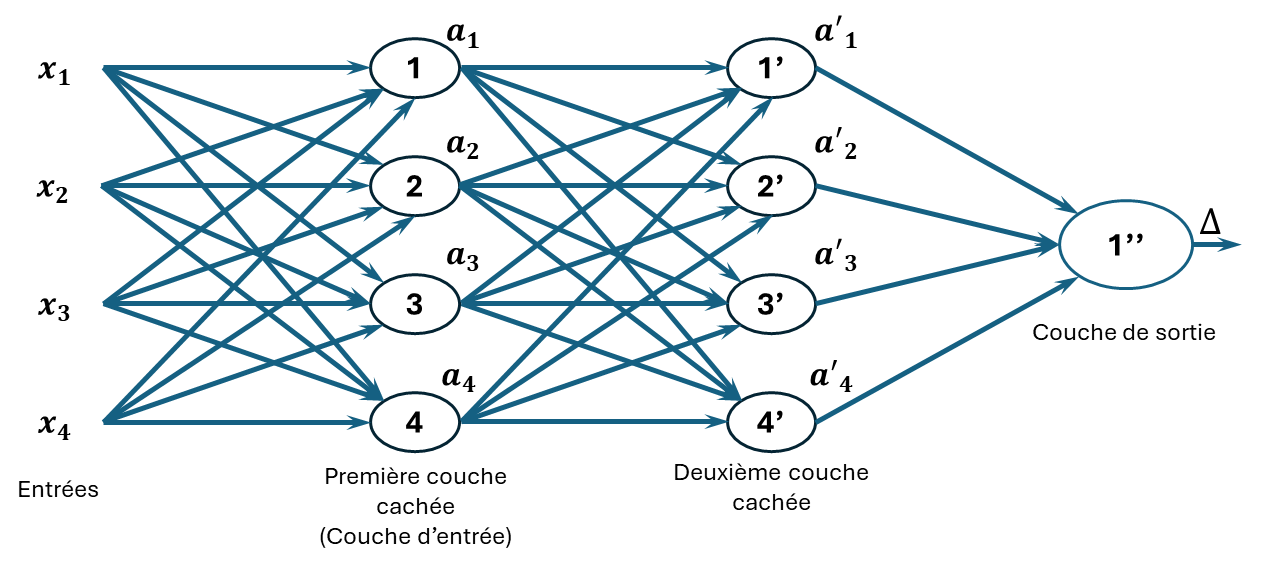
\includegraphics[width=.7\linewidth]{fig_16}
\caption{Structure du réseau de neurones choisi\label{Cy_07_ch_02_td_01_fig_16}}
\end{figure}

Le détail d'un neurone est défini par la figure \ref{Cy_07_ch_02_td_01_fig_17}.

\begin{figure}[!h]
\centering
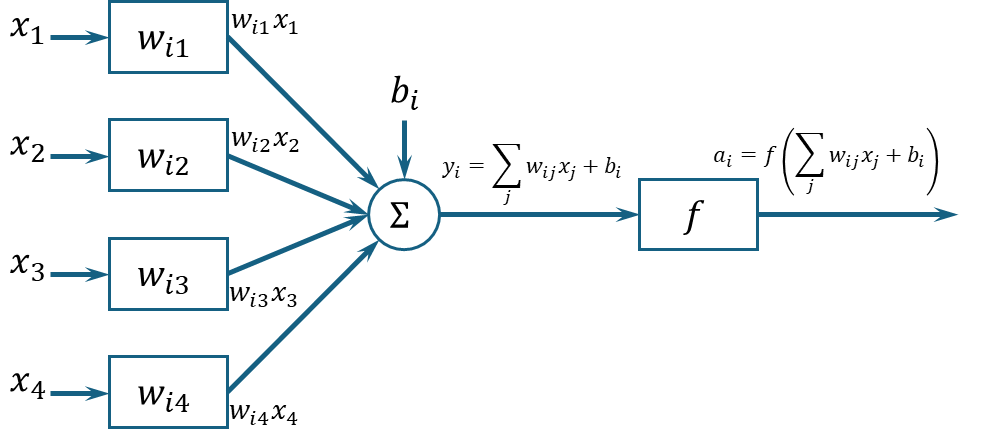
\includegraphics[width=.7\linewidth]{fig_17}
\caption{Structure d'un neurone $i$ de la première couche\label{Cy_07_ch_02_td_01_fig_17}}
\end{figure}

La figure \ref{Cy_07_ch_02_td_01_fig_17} d'un neurone numéroté << $i$ >> de la première couche permet, à partir des valeurs d'entrées $\left(x_1, x_2, x_3, x_4 \right)$ de calculer la valeur de sortie $a_i$. Les sorties de la première couche deviennent les entrées de la couche suivante et ainsi de suite. Tous les neurones vont se comporter cimme ceux de la première couch. Il est à noter que la sortie du dernier neurone correspond à $\Delta$.

\marginnote{Nous noterons :
\begin{itemize}
\item $w_{ij}$ : le poids entre l'entrée $j$et le neurone $i$, c'est un nombre réel;
\item $b_{i}$ : le biais du neurone $i$, c'est un nombre réel; 
\item $f$ : la fonction d'activation du neurone $i$ qui s'applique à $\sum\limits_{j} w_{ij}x_j + b_i$.
\end{itemize}
Le processus permettant de trouvr les valeurs de $b_i$ et de $w_{ij}$ va être itératif. Les valeurs initiales seront choisies aléatoirement.}



La fonction d'activation choisie est une sigmoïde définie par $f: \mathbb{R} \to \mathbb{R}$, $x\to f(x) = \dfrac{1}{1+e^{-x}}$. En Python, l'utilisation de la fonction \lstinline{exp} de la librairie \lstinline{numpy} permet de calculer, pour une entrée \lstinline{X} de type tableau, la matrice $f(x)$, issue de l'application de la fonction $f$ ) tous les éléments de la matrice \lstinline{X}. Cette fonctio d'activation se traduit par la fonction suivante.
\begin{lstlisting}
def f(x) :
    return (1/(1+np.exp(-x)))
\end{lstlisting}


% Q33
\question{Calculer la dérivée de la fonction $f$ notée $f'(x)$ et écrire une fonction Python notée \lstinline{f_prime} qui prend en argument $x$ et qui renvoie la dérivée $f'(x)$. L'argument d'entrée $x$ est de type tableau.}
\ifprof
\begin{corrige}
\end{corrige}
\else
\fi

\subsection*{Phase d'inférence}
%
\marginnote{Notations :
\begin{itemize}
\item les grandeurs scalaires seront notées en minuscule, par exemple $w$;
\item les grandeurs matricielles seront notées en majuscule, par exemple $W$;
\item l'indice $k$ fait référence à la couche, par exemple $W_2$ est pour la deuxième couche. 
\end{itemize}}
%
La phrase d'inférence consiste à calculer la sortie à partir d'un vecteur d'entrée connu. La sortie du dernier neurone du réseau est la valeur $\Delta$ recherché et peut s'écrire sous la forme suivante : 
$\Delta = f\left(W_3\left(f\left(W_2\left(f\left(W_1 X + B_1\right)\right)\right)\right)\right)$.
%

% Q34
\question{Donner les dimensions des matrices $W_3$, $W_2$, $B_2$ et $b_3$.}
\ifprof
\begin{corrige}
\end{corrige}
\else
\fi

On cherche àmodéliser la couche d'entrée du réseau de neurones de la figure \ref{Cy_07_ch_02_td_01_fig_16}. 


% Q35
\question{Donner l'expresiode la matrice $W_1$ qui vérifie :
$$
\begin{pmatrix}
y_1 \\ y_2 \\ y_3 \\ y_4 \\
\end{pmatrix}
=
W_1
\begin{pmatrix}
x_1 \\ x_2 \\ x_3 \\ x_4 \\
\end{pmatrix}
+\begin{pmatrix}
b_1 \\ b_2 \\ b_3 \\ b_4 \\
\end{pmatrix}
 = 
\begin{pmatrix}
- & - & - & -\\
- & - & - & -\\
- & - & - & -\\
- & - & - & -\\
\end{pmatrix}
\begin{pmatrix}
x_1 \\ x_2 \\ x_3 \\ x_4 \\
\end{pmatrix}
+\begin{pmatrix}
b_1 \\ b_2 \\ b_3 \\ b_4 \\
\end{pmatrix}
.$$}
\ifprof
\begin{corrige}
\end{corrige}
\else
\fi

% Q36
\question{Ecrire en Python la fonction \lstinline{inference_couche} qui va prendre en argument le vecteur d'entrées noté $X$, la matrice des points notée $W$, le vecteur biais noté $B$ et qui renvoie le vecteur des sorties de la couche noté $A$ \sidenote{xxx}.}
\ifprof
\begin{corrige}
\end{corrige}
\else
\fi

La figure \ref{Cy_07_ch_02_td_01_fig_18} montre le tracé de la fonction d'activation sigmoïde.

\begin{figure}[!h]
\centering
XXX
%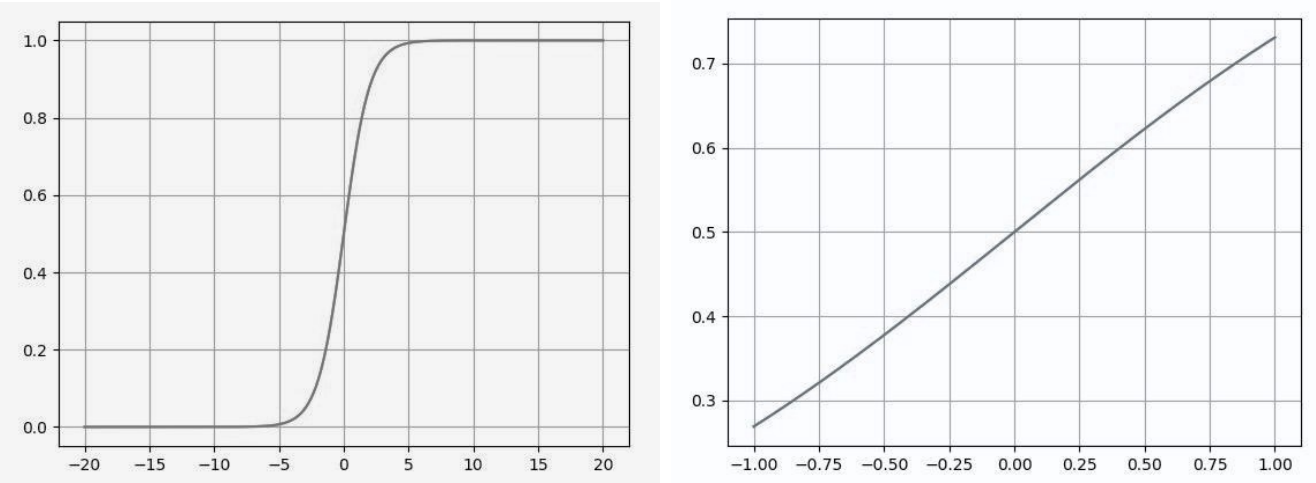
\includegraphics[width=.7\linewidth]{fig_18}
\caption{Représentation graphique de la fonction sigmoïde $f$ pour $x\in [-20,20]$ (à gauche) et $x\in [-1,1]$ (à droite)\label{Cy_07_ch_02_td_01_fig_18}}
\end{figure}

% Q37
\question{Calculer $A=f(Y)$ dans le cas où :
$ A=
\begin{pmatrix}
a_1 \\ a_2 \\ a_3 \\ a_4 \\
\end{pmatrix}$,
$Y=
\begin{pmatrix}
y_1 \\ y_2 \\ y_3 \\ y_4 \\
\end{pmatrix}$,
$X=
\begin{pmatrix}
x_1 \\ x_2 \\ x_3 \\ x_4 \\
\end{pmatrix}=
\begin{pmatrix}
0 \\ 1 \\ 0 \\ 0 \\
\end{pmatrix}$,
$W = 
\begin{pmatrix}
0,3 & 0,2 & 0,25 & -0,03 \\
0,4 & -0,3 & 0,6 & -0,3 \\
-0,4 & 0,3 & -0,6 & -0,5 \\
-1 & -0,75 & -0,1 & -0,5 \\
\end{pmatrix}$,
$B=
\begin{pmatrix}
b_1 \\ b_2 \\ b_3 \\ b_4 \\
\end{pmatrix}=
\begin{pmatrix}
0 \\ 0 \\ 0 \\ 0 \\
\end{pmatrix}
$.}
\ifprof
\begin{corrige}
\end{corrige}
\else
\fi


Notons que, pour cette première phase d'apprentissage qu'on appelle souvent l'initialisation, les valeurs des poids ont été générées aléatoirement et les biais choisis nuls. En reproduisant le même calcul pour les couches suivantes, nous calculons que $\Delta= \SI{0,59}{V}$. Cela signifie que pour l'éclairage allumé et tous les appareils éteints,il faudrait un réglage de $\Delta= \SI{0,59}{V}$.

Cependant le tableau \ref{Cy_07_ch_02_td_01_tab_03} indique que pour cette combinaison d'états, le réglage optimal est $\indice{\Delta}{opt} = \SI{0,18}{V}$.

Il faut modifier les valeurs des poids et des biais pour que la sortie $\Delta$ du réseau de neurons se rapporche de $\indice{\Delta}{opt}$ et ce pour toutes les combinaisons d'entrées possibles. Autrement dit, pour toute combinaison d'entrée $\left(x_1, x_2, x_3, x_4 \right)$, on souhaite minmiser l'erreur (choisie quadratique ici) entre la sortie $\Delta$ calculée par le réseau de neurones et le réglage optimal $\indice{\Delta}{opt}$, déterminé à l'avance. 
Pour ne pas alourdir les notations on notera désormais $t$ le réglage optimal $\indice{\Delta}{opt}$. Le calcul d'erreur $(t-\Delta)^2$ va être utilisé pour calculer des << meilleures >> valeurs de poids et de biais. C'est la phase d'entrainement qui fait partie de la partie suivante.


\subsection*{Rétropropagation \sidenote{REVOIR NOTATIONS}}
Nous disposons de $N=9$ données d'entrainementn c'est-à-dire toutes les paires $\{ X_{\ell},t_{\ell}\}$ où 
$X_{\ell} = \left(x_1, x_2, x_3, x_4 \right)$ est le vecteur de la combinaison des entrées $t_{\ell}$ est simplement la valeur optimale $\indice{\Delta}{opt}$, évaluée empiriquement et qui constitue la valeur cible souhaitée en sortie du réseau de neurones.
 
 Ces données d'entrainement sont recensées dans le tableau \ref{Cy_07_ch_02_td_01_tab_03}. Pour chaque donnée d'entrainement  $\{ X_{\ell},t_{\ell}\}$, on notera $\Delta_t$ le résultat réellement renvoyé par le réseau de neurones. Le but de la phase de rétropropagation est de calculer des valeurs de paramètres 
 $W$ et $B$ qui << rapprochent >> tous les $\Delta_{\ell}$ calculés pour les $X_{\ell}$ des valeurs optimales 
 $t_{\ell}$. Une instance de rétropropagation s'effectue en cherchant les valeurs des paramètres $W$ et $B$ qui minimisent la fonction de coût quadratique entre la cible  $t_{\ell}$ et la valeur calculée 
 $\Delta_{\ell} = \mathcal{L}_{\ell} = \left(t_{\ell} - \Delta_{\ell}\right)^2$.
 
 Pour des raisons de lisibilité, on notera $\mathcal{L} = \mathcal{L}_{\ell}$.

Pour ce faire, les poids $W$ et les biaisn $B$ sont mis à jour par la méthode de la descent du gradient, étudiée dans les questions ci-après. Afin de se fixer les idées, on s'intéresse à la première couche du réseau de neurones, ayant pour entrée le vecteur $X$ et pour sortie le vecteur d'activation $A$ : $A=f\left(W_A X + B_1\right)$. Le fonctionnement des autres couches sera identique. Pour des raisons de lisibilité, on posera désormais $W=W_1$, $B=B_1$, $Y=WX+B$. On a donc : $A = f\left(WX + B\right) = f\left(Y\right)$.

Les valeurs des paramètres $W$ et $B$ de cette couche sont mis à jour grâce aux formules suivantes : 
$\left\{
\begin{array}{l}
W = W -\alpha \dfrac{\partial \mathcal{L}}{\partial W} \\
B = B -\alpha \dfrac{\partial \mathcal{L}}{\partial B}
\end{array}
\right.$

où $\alpha$ est le taux d'apprentissage, un paramètre à choisir manuellement. On adopte la notation suivante :

$ \dfrac{\partial \mathcal{L}}{\partial W} =
\begin{pmatrix}
\dfrac{\partial \mathcal{L}}{\partial w_{11}} & \cdots & \dfrac{\partial \mathcal{L}}{\partial w_{14}} \\
\vdots & \vdots & \vdots \\
\dfrac{\partial \mathcal{L}}{\partial w_{41}} & \cdots & \dfrac{\partial \mathcal{L}}{\partial w_{44}} \\
\end{pmatrix}
$, 
$ \dfrac{\partial \mathcal{L}}{\partial X} =
\begin{pmatrix}
\dfrac{\partial \mathcal{L}}{\partial x_{1}} \\
\vdots \\
\dfrac{\partial \mathcal{L}}{\partial x_{4}} \\
\end{pmatrix}
$, 
$ \dfrac{\partial \mathcal{L}}{\partial A} =
\begin{pmatrix}
\dfrac{\partial \mathcal{L}}{\partial a_{1}} \\
\vdots \\
\dfrac{\partial \mathcal{L}}{\partial a_{4}} \\
\end{pmatrix}
$.

Nous avons 
$\dfrac{\partial \mathcal{L}}{\partial w_{ij}}
=
\dfrac{\partial \mathcal{L}}{\partial a_1} \dfrac{\partial a_1}{\partial w_{ij}}+ \cdots +
\dfrac{\partial \mathcal{L}}{\partial a_i}  \dfrac{\partial a_i}{\partial w_{ij}}+ \cdots +
\dfrac{\partial \mathcal{L}}{\partial a_4} \dfrac{\partial a_4}{\partial w_{ij}}
$ et $a_i = f\left(\sum\limits_{j} w_{ij}x_j + b_i\right)$.

% Q38
\question{ Montrer que 
$ \dfrac{\partial \mathcal{L}}{\partial w_{ij}}
= \dfrac{\partial \mathcal{L}}{\partial a_i} f'(y_i)x_j$.}
\ifprof
\begin{corrige}
\end{corrige}
\else
\fi

% Q39
\question{En utilisant le relation précédente, donner la relation matricielle entre 
$\dfrac{\partial \mathcal{L}}{\partial W}$,
$\dfrac{\partial \mathcal{L}}{\partial A}$,$f'(Y)$ et $X$, puis entre 
$\dfrac{\partial \mathcal{L}}{\partial W}$,
$\dfrac{\partial \mathcal{L}}{\partial A}$, $W$, $X$ et $B$.}
\ifprof
\begin{corrige}
\end{corrige}
\else
\fi

En poursuivant l'analyse il est possible de trouver la relation suivante qui va permettre d'exprimer l'erreur en entrée en fonctiode l'erreur en sortie : 
$ \dfrac{\partial \mathcal{L}}{\partial X} 
= \dfrac{\partial \mathcal{L}}{\partial A} \left(W x f'(WX+B)\right) $\sidenote{xxxx}.

Il est à remarquer que dans la formule précédente, la multiplication se fait terme à terme. 

% Q40
\question{Ecrire la fonction Python \lstinline{retropropagation_couche} qui prend en argument : 
\begin{itemize}
\item la valeur d'entrée d'une couche, notée $X$;
\item la matrice de poids d'une couchen notée $W$;
\item le vecteur de biais de la couche noté $B$;
\item le vecteur d'erreur en sortie de la couche, noté $Ea$;
\item la valeur du coefficient d'apprentissage, notée $\alpha$.
\end{itemize}
Cette fonction doit calculer $E_W = \dfrac{\partial\mathcal{L}}{\partial W}$, 
$E_B = \dfrac{\partial\mathcal{L}}{\partial B}$, 
$E_X = \dfrac{\partial\mathcal{L}}{\partial X}$. 
Cette fonction doit renvoyer : 
\begin{itemize}
\item la matrice de poids $W$ mise à jour;
\item la vecteur de biais $B$ mis à jour;
\item le vecteur gradient du coût $E_x = \dfrac{\partial \mathcal{L}}{\partial X}$.
\end{itemize}
}
\ifprof
\begin{corrige}
\end{corrige}
\else
\fi

% Q31
\question{ }
\ifprof
\begin{corrige}
\end{corrige}
\else
\fi

% Q31
\question{ }
\ifprof
\begin{corrige}
\end{corrige}
\else
\fi

